\documentclass[a4paper,12pt]{report}

\usepackage[italian]{babel}
\usepackage{hyperref}
\usepackage[utf8]{inputenc}
\usepackage{float}
\usepackage[table,xcdraw]{xcolor}
\usepackage{graphicx}

\title{\textbf{CineRadar}\\Progetto di Basi di dati}
\author{Martin Tomassi; 0001077737\\Francesco Pazzaglia; 0001077423\\Luca Casadei; 0001069237}
\date{\today}

\begin{document}
	\maketitle
	\tableofcontents
	\chapter{Analisi dei requisiti}
	\section{Introduzione}
	Il progetto consiste nella realizzazione di un applicativo per la condivisione e la recensione di elementi multimediali quali film e serie TV.
	\section{Intervista}
	È richiesto un sistema che consenta all'utenza di accedere al portale di condivisione di film e serie TV e poter recensirne uno o più di interesse. È necessario che l'utente si registri inserendo i propri dati che verranno salvaguardati, tra cui username, password, nome, cognome, data di nascita per controllare i limiti di età sui film. Un utente deve avere la possibilità di aggiungere nuovi film nel sistema, ma non in maniera diretta, la richiesta deve prima essere approvata da un altro tipo di utente con privilegi di amministratore del sistema. L'amministratore si occuperà di aggiungere film alla piattaforma con frequenza settimanale. Sulle recensioni di altri utenti, un utente può esprimere un parere di utilità che andrà a classificare la recensione in una sorta di "classifica delle recensioni più utili". Quando si va a memorizzare un film bisogna inserire il titolo, uno o più autori, la descrizione, la durata, l'anno di rilascio ed eventuale casa produttrice. I visualizzatori devono essere in grado di vedere tutti i film presenti in base a dei filtri sul genere, categoria, autori e recensioni, sempre a patto che i risultati ottenuti rispettino i limiti di età standard dei film (\textit{over 18, over 16} etc\dots). Quando un utente vede un film della lista, deve poterlo segnare come \textit{"già visto"} per poterlo recensire successivamente se lo desidera. Dato che si vogliono anche incentivare le famiglie, è richiesta una funzionalità che renda possibile inserire un'età e visualizzare i film la cui visione è consentita (per esempio per capire se un film è adatto per il proprio figlio). Un utente registrato all'interno dell'applicativo puó ricevere, in base alla quantità e qualità delle sue recensioni, dei coupon da utilizzare all'interno di un cinema che ha erogato tale sconto, dopo aver ottenuto la loro tessera da affiliato. Il coupon può essere utilizzato per un film o genere specifico entro la sua data di scadenza. Sarà compito dei cinema stabilire quale impiegato avrà la facoltà di erogare le tessere. Per tenere traccia delle strutture che hanno emesso delle tessere vengono memorizzati i cinema attraverso un codice numerico, un indirizzo ed un nome.
	Vi devono essere anche delle piccole classifiche per incentivare gli utenti ad effettuare recensioni, per esempio una classifica degli utenti con il maggior numero di film visualizzati o recensiti. Vi è inoltre una statistica sui film inseriti, per esempio sarà possibile ottenere il genere di film con il maggior numero di visualizzazioni complessive. Oltre che sui film ci devono essere delle statistiche su chi i film li fa, quindi per esempio il regista che ha girato il film con le recensioni migliori e gli eventuali attori che hanno partecipato al cast. L'amministratore può attribuire dei premi in base alla classifica degli utenti migliori (in base alle recensioni più utili), effettuerà anche atti di moderazione sugli utenti registrati, ad esempio, se un utente effettua troppe recensioni al di sotto della soglia di utilità potrà essere rimosso o bloccato dall'effettuare l'accesso al sistema.
	\section{Rielaborazione del testo}
	\subsection{Obiettivi finali:}
	È richiesto un sistema che consenta all'utenza di accedere al portale di condivisione di \textcolor{orange}{\underline{film}} e \textcolor{orange}{\underline{serie TV}} per poterne recensire uno o più di interesse.\\
	Vi devono essere anche delle piccole \textcolor{orange}{\underline{classifiche}} per incentivare gli utenti ad effettuare \textcolor{orange}{\underline{recensioni}}, per esempio una classifica degli utenti con il maggior numero di film visualizzati o recensiti.\\ 
	Vi è inoltre una statistica sui film inseriti, per esempio sarà possibile ottenere il \textcolor{orange}{\underline{genere}} di film con il maggior numero di visualizzazioni complessive. Inoltre è richiesta anche una statistica sugli \textcolor{orange}{\underline{attori}} e i \textcolor{orange}{\underline{registi}} che hanno prodotto i film inseriti, esempio, l'attore con più comparse all'interno dei film inseriti.
	Un utente registrato all'interno dell'applicativo puó ricevere, in base alla quantità e qualità delle sue recensioni, dei coupon da utilizzare all'interno di un cinema che ha erogato tale sconto, dopo aver ottenuto la loro tessera da affiliato. Il coupon puó essere utilizzato per un film o genere specifico entro la sua data di scadenza.
	\subsection{Funzionalità lato utente:}
	È necessario che l'\textcolor{orange}{\underline{utente}} si registri inserendo i propri dati che verranno salvaguardati, tra cui username, password, nome, cognome, data di nascita per controllare i limiti di età sui film. Un utente deve avere la possibilità di aggiungere nuovi \textcolor{orange}{\underline{film}} attraverso una richiesta al sistema, essa deve prima essere approvata da un altro tipo di utente con privilegi di \textcolor{orange}{\underline{amministratore}} del sistema.\\
	Quando un utente vede un film della lista, deve poterlo segnare come \textcolor{orange}{\underline{"Visto"}} per poterlo recensire successivamente se lo desidera. Dato che si vogliono anche incentivare le \textcolor{orange}{\underline{famiglie}}, è richiesta una funzionalità che renda possibile inserire un'età e visualizzare i film la cui visione è consentita (per esempio per capire se un film è adatto per il proprio figlio).\\
	I visualizzatori devono essere in grado di vedere tutti i film presenti in base a dei \textcolor{orange}{\underline{filtri}} sul genere, categoria, autori e recensioni, sempre a patto che i risultati ottenuti rispettino i \textcolor{orange}{\underline{limiti di età}} standard dei film (\textit{over 18, over 16} etc\dots).
	\subsection{Funzionalità lato amministrativo:}
	L'\textcolor{orange}{\underline{amministratore}} si occuperà di aggiungere film alla piattaforma con frequenza settimanale. Sulle recensioni di altri utenti, un utente può esprimere un parere di utilità che andrà a classificare la recensione in una sorta di "classifica delle recensioni più utili".\\
	Quando si va a memorizzare un film bisogna inserire il titolo, uno o più autori, la descrizione, la durata, l'anno di rilascio ed eventuale casa produttrice.
	L'amministratore può attribuire dei \textcolor{orange}{\underline{premi}} in base alla classifica degli utenti migliori (in base alle recensioni più utili), effettuerà anche atti di moderazione sugli utenti registrati, ad esempio, se un utente effettua troppe recensioni al di sotto della soglia di utilità potrà essere rimosso o bloccato dall'effettuare l'accesso al sistema.
	\subsection{Termini da chiarire}\label{ss:terminologia}
	\begin{itemize}
		\item "Utente" $\longrightarrow$ Un utilizzatore dell'applicativo che si registra (o che accede) alla piattaforma ed ha come compito principale la visione, scrittura e valutazione di recensioni.
		\item "Visto" $\longrightarrow$ Un utente può spuntare una casella "visto" se ha visto effettivamente il film, un utente può recensire un film solo se è stato spuntato come "visto".
		\item "Filtro" $\longrightarrow$ Un filtro viene applicato sulla ricerca che può fare un utente sulla lista di film / serie, questo può riguardare l'autore, il titolo, le recensioni dell'utenza etc\dots
		\item "Classifica" $\longrightarrow$ Una lista visualizzabile sull'applicativo in base a parametri scelti; il concetto non viene esplicitato nello schema concettuale ma sarà realizzato attraverso delle query.
		\item "Famiglia" $\longrightarrow$ Un utente genitore può effettuare una sorta di controllo parentale inserendo un'età in un'apposita casella e visualizzando tutti i film che rispettano il limite di età inserito.
		\item "Serie TV" $\longrightarrow$ Sinonimo di film in questo contesto, dato che non vi è alcuna differenza tra i due.
	\end{itemize}
	\section{Estrazione dei dati del testo rielaborato}
	\subsection{Estrazione dati sugli utenti}
	\textbf{Utente} $\longrightarrow$ Utente che si registra sull'applicativo\\Successivamente verranno elencati i dati da dover memorizzare.
	\begin{itemize}
		\item Nome
		\item Cognome
		\item Data di nascita
		\item Username
		\item Password
	\end{itemize}
	\textbf{Amministratore} $\longrightarrow$ Utente privilegiato che effettua operazioni di moderazione e inserimento dati. Dato che nell'intervista non emergono i dati da memorizzare per l'amministratore, si presuppone che vi sia un contatto per poterlo raggiungere, oltre che alle credenziali.
	\begin{itemize}
		\item Username
		\item Password
		\item Nome
		\item Cognome
		\item Telefono
	\end{itemize}
	\subsection{Estrazione dati sui film/serie e produttori}
	\textbf{Film / Serie TV} $\longrightarrow$ Elementi multimediali su cui gli utenti registrati possono apporre la propria visualizzazione ed effettuare recensioni in seguito.
	\begin{itemize}
		\item Data di rilascio
		\item Titolo
		\item Descrizione
		\item Genere
		\item Limite di età
	\end{itemize}
	\textbf{Attori} $\longrightarrow$ Questi vengono memorizzati per stilare la classifica visualizzabile, ed esplicitare delle preferenze. Fanno parte del cast di un film.
	\begin{itemize}
		\item Nome
		\item Cognome
		\item Nome d'arte
		\item Data di nascita
	\end{itemize}
	\textbf{Registi} $\longrightarrow$ Sono coloro che dirigono il cast.
	\begin{itemize}
		\item Nome
		\item Cognome
		\item Data di nascita
		\item Debutto carriera
	\end{itemize}
	\subsection{Elenco delle azioni}
	\subsubsection{Utente}
	\begin{itemize}
		\item Registrarsi sulla piattaforma.
		\item Accedere alla piattaforma.
		\item Scegliere le proprie categorie di preferenza.
		\item Visualizzare i film/serie in base ai filtri scelti e ai limiti di età.
		\item Data un età inferiore alla propria, ottenere la lista dei film che sono visualizzabili con quell'età.
		\item Richiedere all'amministratore l'aggiunta di un film / serie non presente in elenco.
		\item Contrassegnare come visualizzato un film / serie.
		\item Recensire i film contrassegnati come visualizzati.
		\item Dare una valutazione di utilità alle recensioni degli altri utenti.
		\item Ricercare dei film in base al genere o all'autore.
		\item Visualizzare le classifiche degli autori e dei generi.
	\end{itemize}
	\subsubsection{Amministratore}
	\begin{itemize}
		\item Ottenere le statistiche degli utenti registrati alla piattaforma per poter effettuare attività di moderazione, tra cui: 
		\begin{itemize}
			\item (S)Bloccare o eliminare l'accesso ad un utente alla piattaforma se ha effettuato troppe recensioni che stanno sotto alla soglia di utilità.
			\item Premiare l'utente in cima alla classifica delle recensioni più utili (il premio è una targhetta che comparirà accanto al nome).
		\end{itemize}
		\item Aggiungere film / serie alla lista, compresi quelli che sono stati richiesti dagli utenti.
		\item Inserire nuovi autori o registi da associare a dei film.
	\end{itemize}
	\chapter{Progettazione concettuale}
	\section{Strategia bottom-up}
	\subsection{Utenza}
	Rappresentazione di una sottoparte dello schema ER che riguarda la gestione dell'utenza, in particolare, è stata pensata una generalizzazione dell'entità \textbf{utilizzatore} con due sotto-entità \textbf{amministratore} e \textbf{utente} di cui dobbiamo memorizzare elementi diversi. La generalizzazione è di tipo \textit{totale} e \textit{esclusiva}, questo perché l'amministratore ha un tipo di account diverso da quello di semplice utente, se l'amministratore vuole effettuare le operazioni di un utente normale deve registrarsi con un altro account.
	\begin{figure}[H]
		\centering
		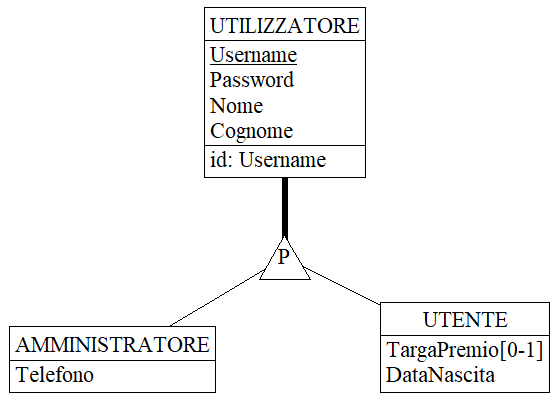
\includegraphics[width=250pt]{ER/utenza.png}
		\caption{Schema ER dell'utenza.}
	\end{figure}
	\subsection{Film}
	Qui viene descritta la rappresentazione di un \textbf{film} / serie, che come si può vedere nel glossario in particolare nella sezione \ref{ss:terminologia} sono lo stesso concetto, quindi non è necessaria una generalizzazione. Un film può essere associato a diversi \textbf{generi}, \textit{(quindi esistono film che sono sia horror che commedia per esempio)}, e l'inserimento dei generi è indipendente dall'esistenza dei film, quindi si è optato per la cardinalità \textbf{0-N}.
	\begin{figure}[H]
		\centering
		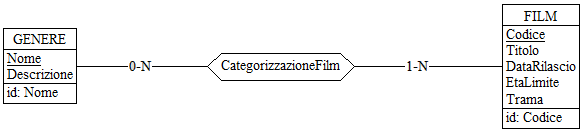
\includegraphics[width=450pt]{ER/film.png}
		\caption{Schema ER dei film.}
	\end{figure}
	\subsection{Cast}
	I membri del cast da tracciare possono essere \textbf{registi} o \textbf{attori}; degli attori ci interessa in particolare un nome d'arte, mentre dei registi la data di debutto della carriera per effettuare delle statistiche. La generalizzazione in questo caso è \textit{totale} e \textit{sovrapposta}, questo significa che nel dominio del nostro problema non si vogliono tracciare altri membri oltre che a questi due, ed è sovrapposta perché possono esserci casi in cui un regista è anche un attore.
	\begin{figure}[H]
		\centering
		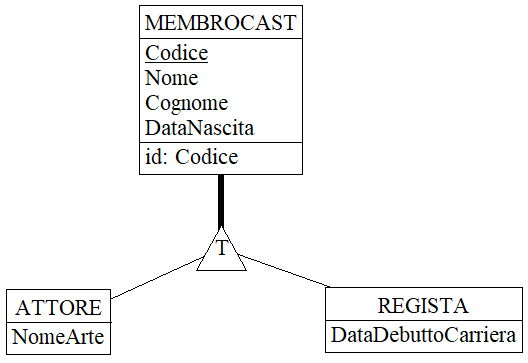
\includegraphics[width=250pt]{ER/cast.png}
		\caption{Schema ER dei membri del cast.}
	\end{figure}
	
	\subsection{Coupon}
	Un coupon rappresenta un'offerta promozionale, espressa come una percentuale di sconto, che può essere utilizzata da un Utente. Viene suddiviso in due sotto entità in maniera totale ed esclusiva:
	\begin{itemize}
			\item Coupon singolo: si riferisce ad uno e un solo film.
			\item Coupon multiplo: si riferisce ad uno o più generi di film.
	\end{itemize}
	\begin{figure}[H]
		\centering
		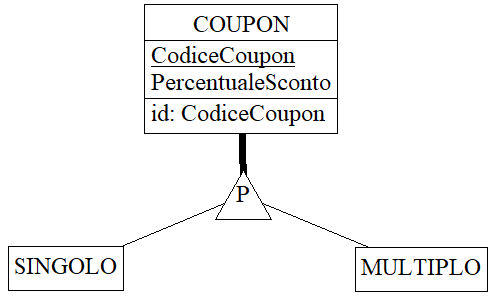
\includegraphics[width=250pt]{ER/coupon.png}
		\caption{Schema ER del coupon.}
	\end{figure}
	\subsection{Relazione tra registratore e tessera}
	Il testo esplicita come una tessera predisponga di un nome e di una relativa scadenza. La tessera deve essere inserita e nel sistema da parte di un gestore del cinema che la emette, questo gestore avrà quindi un account di accesso a parte. Un gestore è associato per forza di cose ad uno e un solo cinema, quindi se una persona lavora in più cinema e in entrambi può rilasciare tessere avrà due account con credenziali diverse.
	\begin{figure}[H]
		\centering
		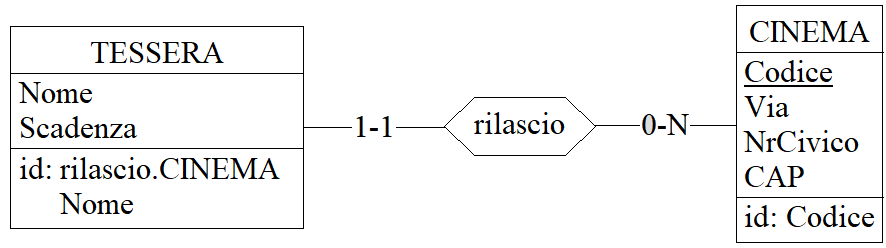
\includegraphics[width=0.7\linewidth]{ER/cinetessera.png}
		\caption{Schema ER della relazione tra il cinema e la tessera.}
	\end{figure}
	\subsection{Relazione tra utenza e recensioni}
	Il testo esplicita come un utente può scrivere piú di una recensione su vari film, esplicitando il titolo del film, la descrizione della recensione e la sua valutazione. Inoltre, un utente può classificare, tramite un voto di utilitá, piú di una recensione scritta da un altro utente.
	\begin{figure}[H]
		\centering
		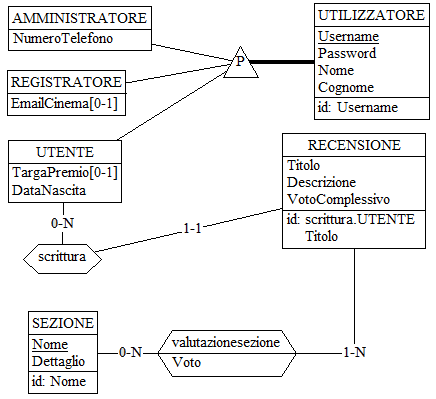
\includegraphics[width=250pt]{ER/utenzarecensione.png}
		\caption{Schema ER della relazione tra utenza e recensioni.}
	\end{figure}
	\subsection{Relazione tra cinema, tessera e coupon}
	Il testo esplicita l'associazione di più promozioni a una singola tessera, e viceversa, consentendo a ciascuna promozione di essere collegata a più tessere. In questa struttura, una promozione è considerata come un legame con coupon. La distinzione tra coupon e promozione risiede nel fatto che il coupon identifica la tipologia di beneficio, mentre la promozione aggiunge a esso una data di scadenza prefissata.
	\begin{figure}[H]
		\centering
		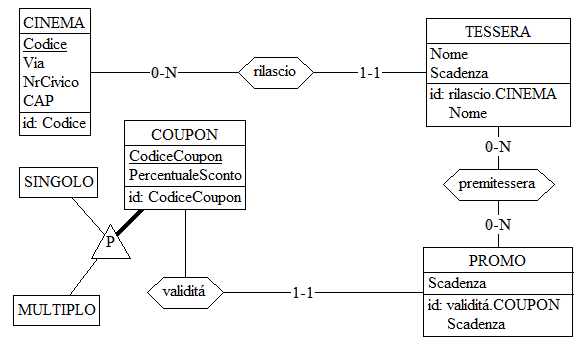
\includegraphics[width=0.7\linewidth]{ER/cinetesseracoupon.png}
		\caption{Schema ER della relazione tra il cinema, la tessera e il coupon.}
	\end{figure}
	\subsection{Relazione tra membri del cast e film}
	Il testo esplicita come di un film dobbiamo memorizzare gli attori che hanno partecipato al cast, e il regista, quindi il regista è uno solo per film e generalmente è così, per questo si spiega la scelta della cardinalità \textbf{1-N} nella relazione con il regista mentre \textbf{N-N} per quella con gli attori.
	\begin{figure}[H]
		\centering
		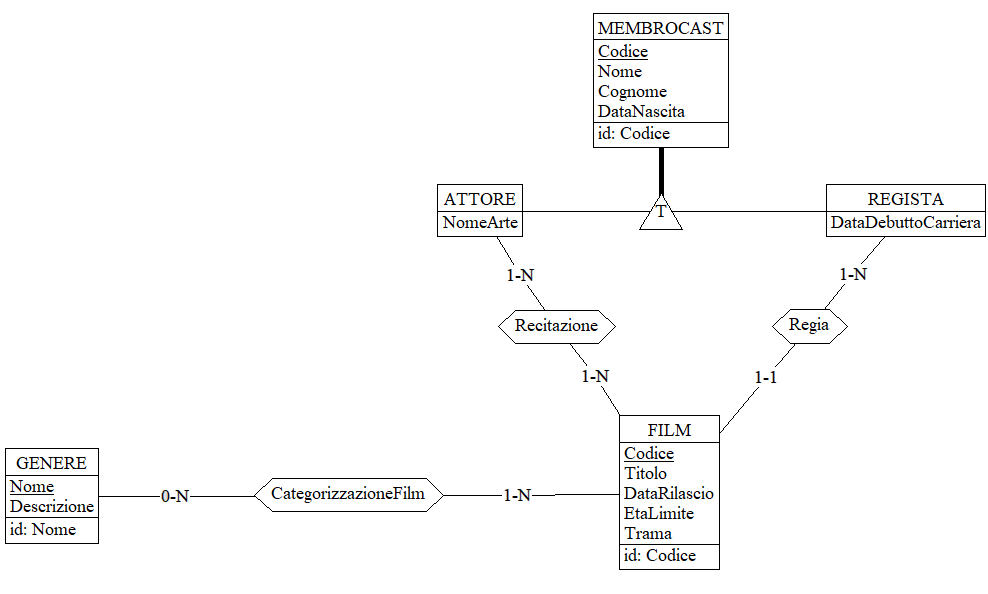
\includegraphics[width=450pt]{ER/filmcast.png}
		\caption{Schema ER della relazione tra membri del cast e film.}
	\end{figure}
	\subsection{Relazione tra film, coupon e tessera}
	Il testo esplicita che: sia un coupon singolo che uno multiplo possono essere utilizzati per ottenere uno sconto su un film in particolare(qualora fosse un coupon singolo) oppure in base al genere del film(nel caso di un coupon multiplo).
	\begin{figure}[H]
		\centering
		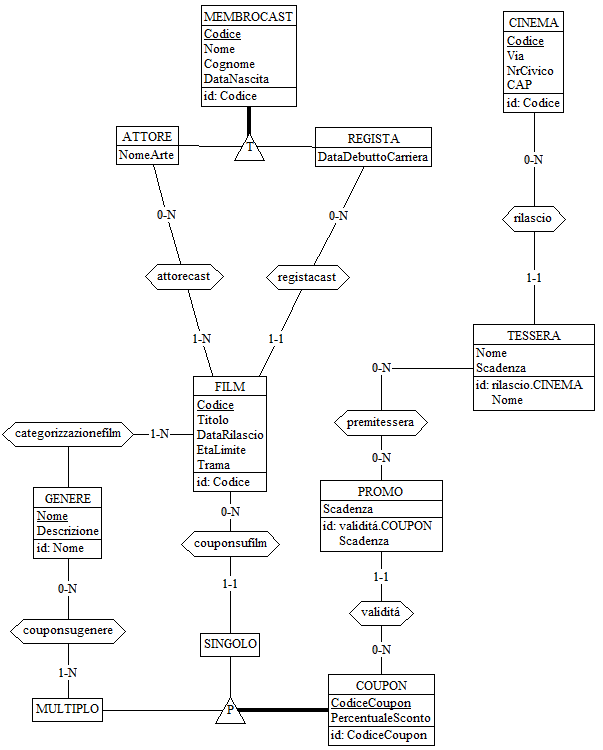
\includegraphics[width=0.9\linewidth]{ER/filmcoupontessera.png}
		\caption{Schema ER della relazione tra il film, il coupon e la tessera.}
	\end{figure}
	\subsection{Schema completo}
	Questo é lo schema derivato dalla composizione di tutte le sotto-componenti descritte precedentemente. Il collegamento tra film e recensione impone che ci sia un unica recensione per film e che quest'ultimo può averne più di una.
	\begin{figure}[H]
		\centering
		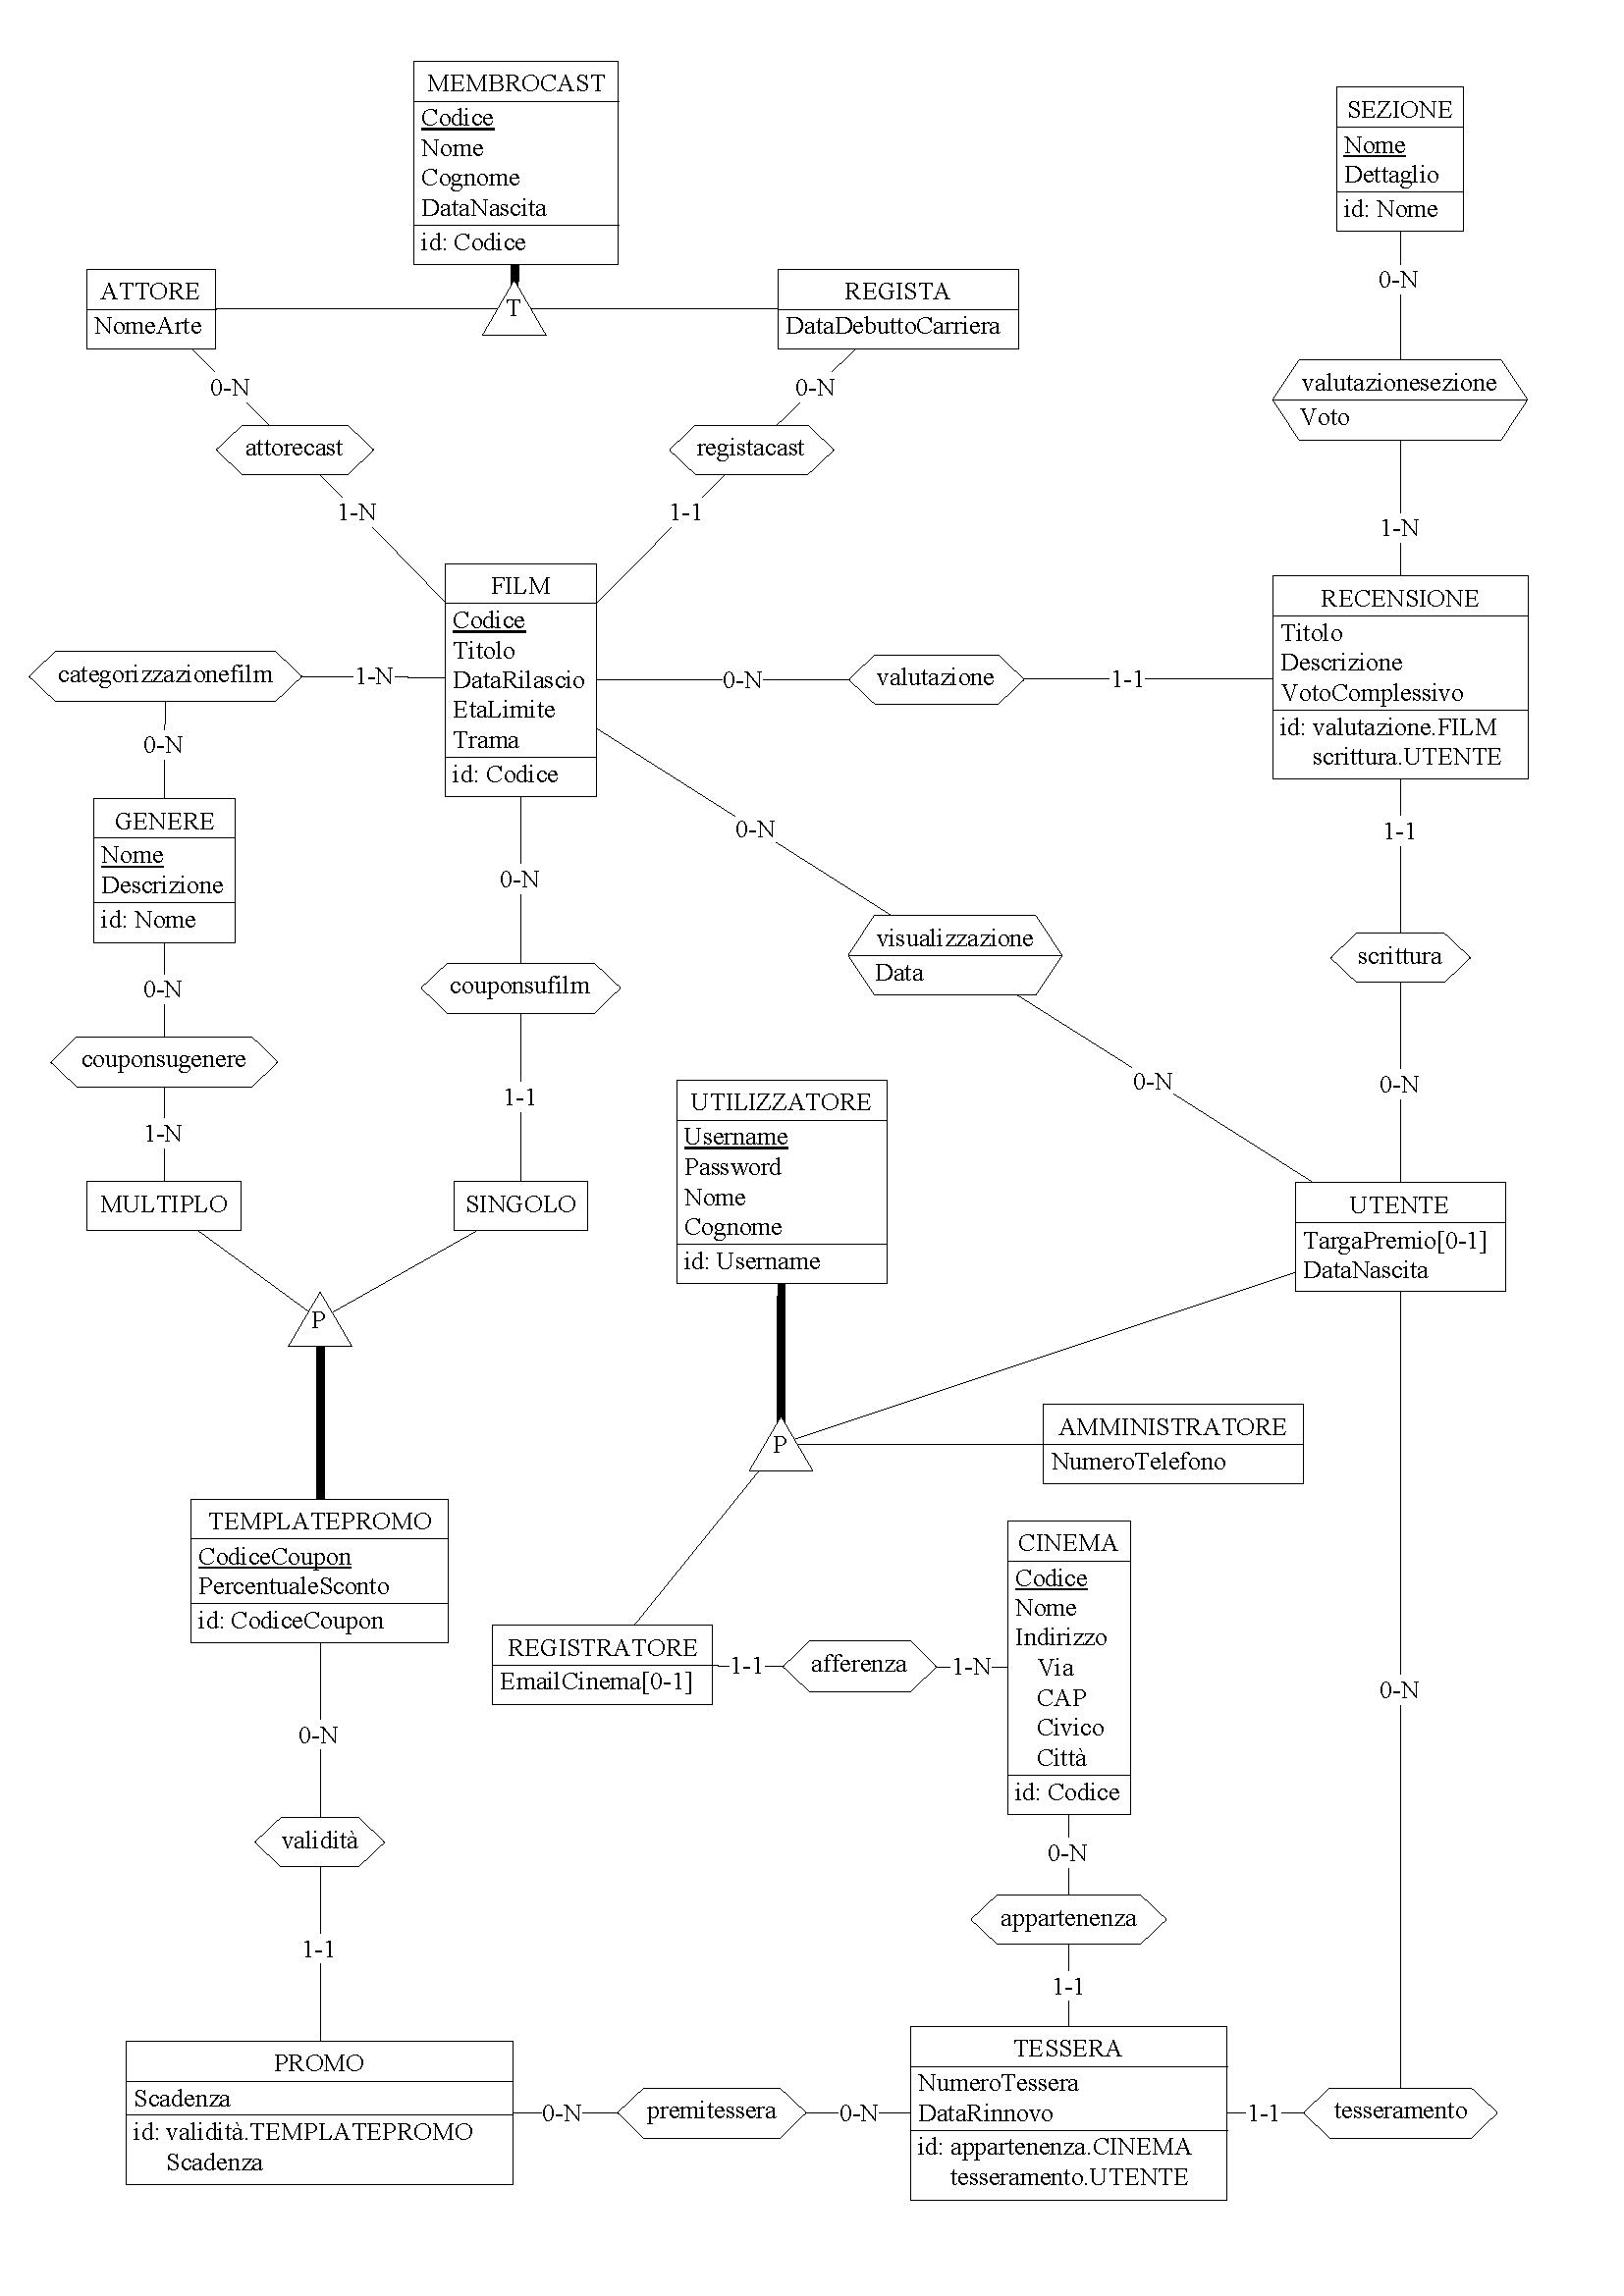
\includegraphics[width=470pt]{ER/ercompleto.png}
		\caption{Schema ER completo.}
	\end{figure}
	\chapter{Progettazione Logica}
	\section{Stima del volume dei dati}
\end{document}